\documentclass{article}
\usepackage{listings}
\usepackage{graphicx}
\usepackage{epstopdf}
\usepackage[english]{babel}

\title{Centralized Chat System}
\author{NGUYEN Vu Bao Hung}
\date{April 8 2018}
\lstset{breaklines=true} 

\begin{document}
\maketitle

\section{Introduction}
In this project, I will develope a chat programme that acts as a chat room. One client can send message to and receive message from all other clients.\\
The system works with non-blocking multiplex TCP socket.

\section{Compiling options}
I use region pragmas in my code for better code view experience, hence it might raise some warnings, please use the following option when compiling to suppress those warnings.\\
-Wno-unknown-pragmas\\
The client and server are multi-threaded with pthread so it is necessary to use the below option while compiling.\\
-pthread\\

\section{The Client}
The client programme is separated into 2 threads, one for handling input and one for displaying messages. This helps user to see new messages as they come and let them send message at any time.\\
The main thread will continue to wait for incoming message.\\
The input thread will wait for user input.\\
The network thread will send the user input to server.\\
The input thread and network thread are synchronized by a mutex such that once the input message is received, it is sent to server.

\section{The Server}
There are 2 versions of the server, single-process and multi-process. Both of them works as expected.\\

\textbf{Version 1: single-process}\\
All clients are managed by one process, once a message is received, it is sent to all other clients.\\

\textbf{Version 2: multi-process}\\
In this version, the parent process handle new connections, the child processes receive and send message to each client.\\
Their will be a different child process for each client.\\
There are 2 pipes for each child-parent pair.\\
The child process will read from Pipe 1 and write to pipe 2.\\
The parent process will write to Pipe 1 and read from Pipe 2.\\

The child will first receive a message from its client. That message is then sent to the parent process through a pipe.\\
Once the parent receive a message from a child, it will send that message to all other children processes.\\
When a child process receive a message from the parent process, it will forward the message to its client.\\

The flow of a message is as followed: Client ==> Server (Child process) ==> Server (Parent process) ==> Server (All other children processes) ==> Clients\\

\textbf{Demonstration}\\
The screenshot below shows a brief picture of the programme.\\

\begin{center}
  \makebox[\textwidth]{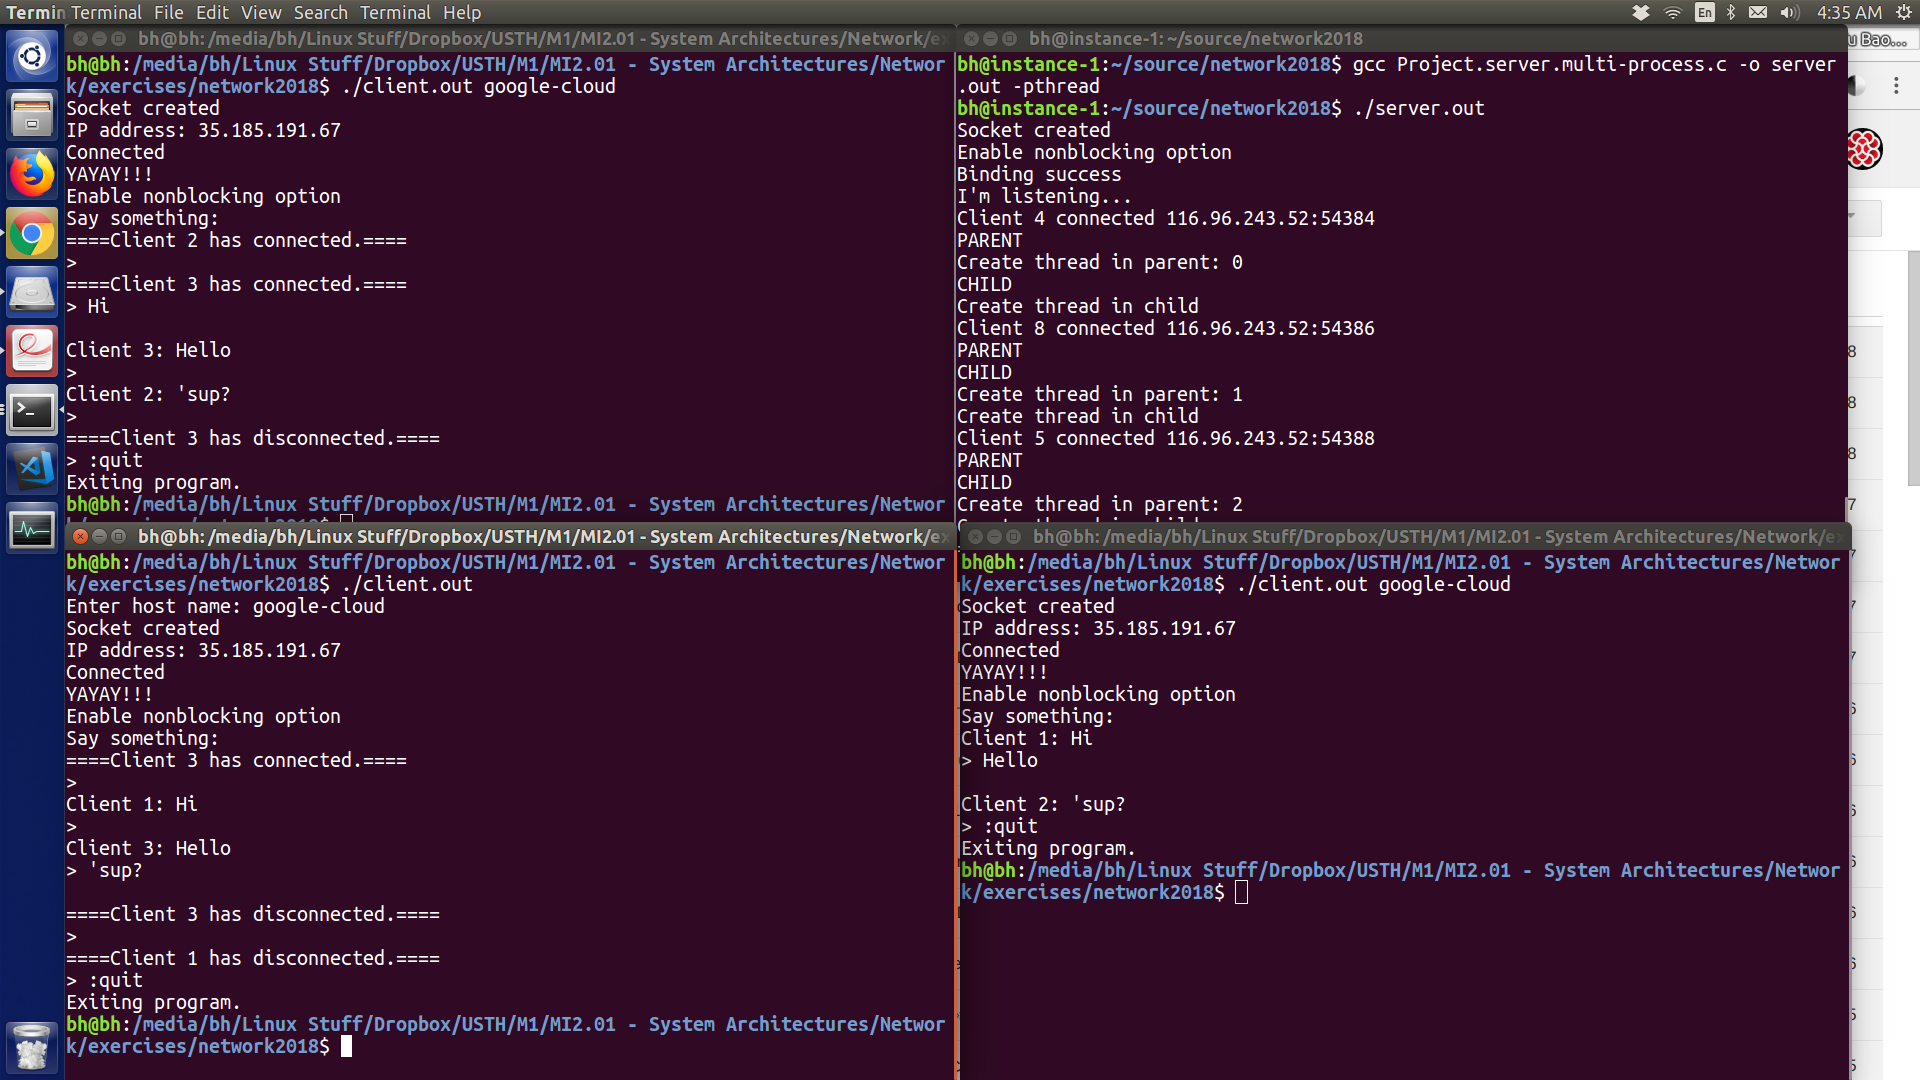
\includegraphics[width=\paperwidth]{Example.png}}
\end{center}

\end{document}